% ============================================================
% 讲义 — 人教版七年级下册 第6章 实数
% 编译命令：xelatex -interaction=nonstopmode 第6章_实数.tex
% ============================================================
\documentclass[12pt, a4paper]{ctexart}
\usepackage[margin=2.2cm]{geometry}
\usepackage{amsmath, amssymb}
\usepackage{enumitem}
\usepackage{tcolorbox}
\usepackage{booktabs}
\usepackage{array}
\usepackage{fancyhdr}
\usepackage{xcolor}
\usepackage{tikz}
\usepackage{hyperref}
\usepackage{graphicx}
\usepackage{multirow}
\usepackage{pgfplots}
\pgfplotsset{compat=1.18}

% 颜色定义
\definecolor{mainblue}{RGB}{41, 98, 168}
\definecolor{lightblue}{RGB}{230, 240, 255}
\definecolor{tipgreen}{RGB}{34, 139, 87}
\definecolor{lightgreen}{RGB}{235, 250, 240}
\definecolor{warnred}{RGB}{200, 50, 50}
\definecolor{lightred}{RGB}{255, 240, 240}
\definecolor{examorange}{RGB}{210, 120, 20}
\definecolor{lightorange}{RGB}{255, 248, 235}
\definecolor{apppurple}{RGB}{120, 60, 170}
\definecolor{lightpurple}{RGB}{245, 238, 255}

% 页眉页脚
\pagestyle{fancy}
\fancyhf{}
\fancyhead[L]{\small\textcolor{mainblue}{\textbf{人教版七年级下册 · 第6章}}}
\fancyhead[R]{\small\textcolor{mainblue}{实数讲义}}
\fancyfoot[C]{\small —\ \thepage\ —}
\renewcommand{\headrulewidth}{0.6pt}
\renewcommand{\headrule}{\hbox to\headwidth{\color{mainblue}\leaders\hrule height \headrulewidth\hfill}}
\renewcommand{\footrulewidth}{0pt}

% tcolorbox 样式
\newtcolorbox{knowledgebox}[1][]{%
  colback=lightblue, colframe=mainblue,
  fonttitle=\bfseries\large, title=#1,
  arc=3mm, boxrule=0.8pt,
  left=8pt, right=8pt, top=6pt, bottom=6pt
}

\newtcolorbox{tipbox}[1][]{%
  colback=lightgreen, colframe=tipgreen,
  fonttitle=\bfseries, title=#1,
  arc=2mm, boxrule=0.6pt,
  left=6pt, right=6pt, top=4pt, bottom=4pt
}

\newtcolorbox{warnbox}[1][]{%
  colback=lightred, colframe=warnred,
  fonttitle=\bfseries, title=#1,
  arc=2mm, boxrule=0.6pt,
  left=6pt, right=6pt, top=4pt, bottom=4pt
}

\newtcolorbox{examplebox}[1][]{%
  colback=lightorange, colframe=examorange,
  fonttitle=\bfseries, title=#1,
  arc=3mm, boxrule=0.8pt,
  left=8pt, right=8pt, top=6pt, bottom=6pt
}

\newtcolorbox{appbox}[1][]{%
  colback=lightpurple, colframe=apppurple,
  fonttitle=\bfseries, title=#1,
  arc=3mm, boxrule=0.8pt,
  left=8pt, right=8pt, top=6pt, bottom=6pt
}

\setCJKmainfont{Hiragino Sans GB}
\setCJKsansfont{Heiti SC}

\begin{document}

% ============ 标题页 ============
\begin{center}
{\Huge\bfseries\textcolor{mainblue}{第6章\quad 实数}}\\[12pt]
{\Large\textcolor{gray}{讲\quad 义}}\\[8pt]
\rule{0.6\textwidth}{1pt}\\[8pt]
{\normalsize 适用：人教版\quad 七年级下册\quad |\quad 课时：5课时}
\end{center}
\vspace{10pt}

% =============================================================
% 第一部分：知识点讲解
% =============================================================
\section*{\textcolor{mainblue}{一、知识点讲解}}

\subsection*{6.1\quad 平方根}

\begin{knowledgebox}[1.\quad 平方根的定义]
如果一个数 $x$ 的平方等于 $a$，即 $x^2 = a$，那么 $x$ 叫做 $a$ 的\textbf{平方根}（也叫二次方根）。

\begin{itemize}[leftmargin=2em]
  \item 一个\textbf{正数}有两个平方根，它们互为相反数。记作 $\pm\sqrt{a}$。
  \item \textbf{0} 的平方根是 0。$\sqrt{0} = 0$。
  \item \textbf{负数}没有平方根（在实数范围内）。
\end{itemize}

例如：$(\pm 3)^2 = 9$，所以 9 的平方根是 $\pm 3$，记作 $\pm\sqrt{9} = \pm 3$。
\end{knowledgebox}

\begin{knowledgebox}[2.\quad 算术平方根]
一个正数 $a$ 的\textbf{正的}平方根叫做 $a$ 的\textbf{算术平方根}，记作 $\sqrt{a}$。

\begin{itemize}[leftmargin=2em]
  \item $\sqrt{a} \geq 0$（算术平方根是非负数）。
  \item 规定：0 的算术平方根是 0，即 $\sqrt{0} = 0$。
  \item $\sqrt{a}$ 中 $a \geq 0$（被开方数必须非负）。
\end{itemize}

例如：$\sqrt{16} = 4$（不是 $\pm 4$），$\sqrt{25} = 5$。
\end{knowledgebox}

\begin{warnbox}[易错提醒]
\begin{itemize}[leftmargin=2em]
  \item $\sqrt{a}$ 表示算术平方根，\textbf{只有正值}（或零）。例如 $\sqrt{9} = 3$，不是 $\pm 3$。
  \item 求"9 的平方根"要答 $\pm 3$；求"$\sqrt{9}$"要答 $3$。两句话含义不同！
  \item $\sqrt{a^2} = |a|$，不是 $a$。例如 $\sqrt{(-5)^2} = \sqrt{25} = 5 \neq -5$。
\end{itemize}
\end{warnbox}

\subsection*{6.2\quad 立方根}

\begin{knowledgebox}[3.\quad 立方根的定义]
如果一个数 $x$ 的立方等于 $a$，即 $x^3 = a$，那么 $x$ 叫做 $a$ 的\textbf{立方根}（也叫三次方根）。记作 $\sqrt[3]{a}$。

\begin{itemize}[leftmargin=2em]
  \item \textbf{正数}有一个正的立方根。
  \item \textbf{负数}有一个负的立方根。
  \item \textbf{0} 的立方根是 0。
\end{itemize}

例如：$\sqrt[3]{8} = 2$，$\sqrt[3]{-8} = -2$，$\sqrt[3]{0} = 0$。

\textbf{重要性质}：$\sqrt[3]{-a} = -\sqrt[3]{a}$（可以将负号提到根号外面）。
\end{knowledgebox}

\begin{tipbox}[平方根与立方根的对比]
\begin{center}
\renewcommand{\arraystretch}{1.4}
\begin{tabular}{lcc}
\toprule
 & \textbf{平方根} & \textbf{立方根} \\
\midrule
正数 & 两个（$\pm\sqrt{a}$） & 一个正的（$\sqrt[3]{a}$） \\
0   & 0 & 0 \\
负数 & 没有（实数范围内） & 一个负的（$\sqrt[3]{a}$） \\
符号 & $\sqrt{a}$（算术平方根） & $\sqrt[3]{a}$ \\
\bottomrule
\end{tabular}
\end{center}
\end{tipbox}

\subsection*{6.3\quad 无理数与实数}

\begin{knowledgebox}[4.\quad 无理数]
\textbf{无理数}：\textbf{无限不循环小数}叫做无理数。

常见的无理数：
\begin{itemize}[leftmargin=2em]
  \item 开方开不尽的数：$\sqrt{2}$，$\sqrt{3}$，$\sqrt{5}$，$\sqrt[3]{2}$ 等。
  \item 特殊常数：$\pi = 3.14159265\ldots$
  \item 人为构造的无限不循环小数：$0.101001000100001\ldots$（相邻两个 1 之间 0 的个数逐次加 1）
\end{itemize}

\textbf{注意}：$\frac{22}{7}$ 不是 $\pi$，$\frac{22}{7}$ 是有理数（分数），$\pi$ 是无理数。
\end{knowledgebox}

\begin{knowledgebox}[5.\quad 实数及其分类]
\textbf{实数}：有理数和无理数统称为实数。

\[
\text{实数}
\begin{cases}
\text{有理数}
\begin{cases}
\text{整数}
\begin{cases}
\text{正整数} \\[2pt]
0 \\[2pt]
\text{负整数}
\end{cases} \\[6pt]
\text{分数（有限小数或无限循环小数）}
\end{cases} \\[10pt]
\text{无理数}（\text{无限不循环小数}）
\end{cases}
\]

实数按符号分类：
\[
\text{实数}
\begin{cases}
\text{正实数}（正有理数 + 正无理数） \\[2pt]
0 \\[2pt]
\text{负实数}（负有理数 + 负无理数）
\end{cases}
\]
\end{knowledgebox}

\begin{knowledgebox}[6.\quad 实数与数轴]
\textbf{实数与数轴上的点一一对应}：
\begin{itemize}[leftmargin=2em]
  \item 每一个实数都可以用数轴上的\textbf{唯一一个点}来表示。
  \item 数轴上的\textbf{每一个点}都表示\textbf{唯一一个实数}。
\end{itemize}

\begin{center}
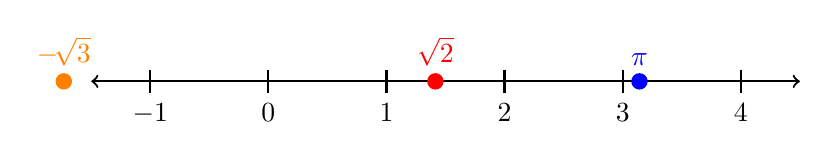
\begin{tikzpicture}[scale=1.5]
  \draw[thick, ->] (-0.5,0) -- (4.5,0);
  \foreach \x/\label in {0/0, 1/1, 2/2, 3/3, 4/4}
    \draw[thick] (\x, 0.1) -- (\x, -0.1) node[below] {$\label$};
  % 标记 sqrt2 的位置（约1.414）
  \draw[thick, red, fill=red] (1.414, 0) circle (0.06);
  \node[above, red] at (1.414, 0.05) {$\sqrt{2}$};
  % 标记 pi 的位置（约3.14159）
  \draw[thick, blue, fill=blue] (3.142, 0) circle (0.06);
  \node[above, blue] at (3.142, 0.05) {$\pi$};
  % 标记 -sqrt3 的位置
  \draw[thick, green!60!black, fill=green!60!black] (-0.5,0);
  % 画负方向
  \draw[thick, ->] (0,0) -- (-1.5,0);
  \foreach \x/\label in {-1/-1}
    \draw[thick] (\x, 0.1) -- (\x, -0.1) node[below] {$\label$};
  \draw[thick, orange, fill=orange] (-1.732, 0) circle (0.06);
  \node[above, orange] at (-1.732, 0.05) {$-\!\sqrt{3}$};
\end{tikzpicture}
\end{center}

数轴上的点与实数一一对应，使得我们可以在数轴上直观地表示无理数。
\end{knowledgebox}

\subsection*{6.4\quad 实数的运算}

\begin{knowledgebox}[7.\quad 实数的运算]
实数可以进行加、减、乘、除（除数不为 0）、乘方运算。

\textbf{有理数的运算律和运算性质在实数范围内仍然适用}。

\textbf{根式的简单运算}：
\begin{enumerate}[leftmargin=2em]
  \item $\sqrt{a} \cdot \sqrt{b} = \sqrt{ab}$\quad（$a \geq 0$，$b \geq 0$）
  \item $\dfrac{\sqrt{a}}{\sqrt{b}} = \sqrt{\dfrac{a}{b}}$\quad（$a \geq 0$，$b > 0$）
  \item $(\sqrt{a})^2 = a$\quad（$a \geq 0$）
  \item $\sqrt{a^2} = |a|$
\end{enumerate}

\textbf{同类根式}可以合并：$2\sqrt{3} + 3\sqrt{3} = 5\sqrt{3}$。
\end{knowledgebox}

\begin{warnbox}[根式运算易错点]
\begin{itemize}[leftmargin=2em]
  \item $\sqrt{a} + \sqrt{b} \neq \sqrt{a+b}$！例如 $\sqrt{9} + \sqrt{16} = 3 + 4 = 7$，而 $\sqrt{9+16} = \sqrt{25} = 5$，$7 \neq 5$。
  \item $\sqrt{a} \cdot \sqrt{b} = \sqrt{ab}$ 要求 $a \geq 0$，$b \geq 0$。
  \item 化简 $\sqrt{12}$ 时：$\sqrt{12} = \sqrt{4 \times 3} = 2\sqrt{3}$，不是 $6\sqrt{2}$。
\end{itemize}
\end{warnbox}

\begin{tipbox}[估算无理数的大小]
估算 $\sqrt{n}$ 在哪两个整数之间：
\begin{itemize}[leftmargin=2em]
  \item 找到 $n$ 前后的两个完全平方数。例如 $\sqrt{10}$：因为 $3^2 = 9 < 10 < 16 = 4^2$，所以 $3 < \sqrt{10} < 4$。
  \item $\sqrt{10} \approx 3.16$（更精确的估计可以用计算器）。
\end{itemize}
常见值：$\sqrt{2} \approx 1.414$，$\sqrt{3} \approx 1.732$，$\sqrt{5} \approx 2.236$。
\end{tipbox}

% =============================================================
% 第二部分：例题精讲
% =============================================================
\section*{\textcolor{examorange}{二、例题精讲}}

\begin{examplebox}[【例题1】求平方根与算术平方根]
求下列各数的平方根和算术平方根：
\begin{enumerate}[label=(\arabic*)]
  \item $36$
  \item $\dfrac{4}{25}$
  \item $0.49$
\end{enumerate}
\end{examplebox}

\textbf{解}：

\begin{enumerate}[label=(\arabic*)]
  \item 因为 $(\pm 6)^2 = 36$，所以 36 的平方根是 $\pm 6$，即 $\pm\sqrt{36} = \pm 6$。

  36 的算术平方根是 $6$，即 $\sqrt{36} = 6$。

  \item 因为 $\left(\pm\dfrac{2}{5}\right)^2 = \dfrac{4}{25}$，所以 $\dfrac{4}{25}$ 的平方根是 $\pm\dfrac{2}{5}$。

  算术平方根是 $\dfrac{2}{5}$，即 $\sqrt{\dfrac{4}{25}} = \dfrac{2}{5}$。

  \item 因为 $(\pm 0.7)^2 = 0.49$，所以 $0.49$ 的平方根是 $\pm 0.7$。

  算术平方根是 $0.7$，即 $\sqrt{0.49} = 0.7$。
\end{enumerate}

\vspace{6pt}

\begin{examplebox}[【例题2】求立方根]
求下列各数的立方根：
\begin{enumerate}[label=(\arabic*)]
  \item $27$
  \item $-64$
  \item $\dfrac{8}{125}$
\end{enumerate}
\end{examplebox}

\textbf{解}：

\begin{enumerate}[label=(\arabic*)]
  \item 因为 $3^3 = 27$，所以 $\sqrt[3]{27} = 3$。

  \item 因为 $(-4)^3 = -64$，所以 $\sqrt[3]{-64} = -4$。

  也可以：$\sqrt[3]{-64} = -\sqrt[3]{64} = -4$。

  \item 因为 $\left(\dfrac{2}{5}\right)^3 = \dfrac{8}{125}$，所以 $\sqrt[3]{\dfrac{8}{125}} = \dfrac{2}{5}$。
\end{enumerate}

\vspace{6pt}

\begin{examplebox}[【例题3】判断有理数与无理数]
将下列各数分类：

\[
\sqrt{7},\quad -\frac{3}{4},\quad 0,\quad \sqrt[3]{-27},\quad \pi,\quad 0.\overline{3},\quad \sqrt{16},\quad 0.1010010001\ldots
\]

哪些是有理数？哪些是无理数？
\end{examplebox}

\textbf{解}：

\textbf{有理数}：$-\dfrac{3}{4}$，$0$，$\sqrt[3]{-27} = -3$，$0.\overline{3}$（循环小数），$\sqrt{16} = 4$。

\textbf{无理数}：$\sqrt{7}$，$\pi$，$0.1010010001\ldots$（无限不循环小数）。

\begin{warnbox}[易错提醒]
$\sqrt[3]{-27} = -3$ 是有理数（整数），$\sqrt{16} = 4$ 是有理数（整数）。判断时要先化简，再分类！
\end{warnbox}

\vspace{6pt}

\begin{examplebox}[【例题4】估算无理数的大小]
估算 $\sqrt{20}$ 在哪两个连续整数之间，并精确到十分位。
\end{examplebox}

\textbf{解}：

因为 $4^2 = 16 < 20 < 25 = 5^2$，

所以 $4 < \sqrt{20} < 5$。

进一步估算：
\begin{itemize}[leftmargin=2em]
  \item $4.4^2 = 19.36 < 20$
  \item $4.5^2 = 20.25 > 20$
\end{itemize}

所以 $4.4 < \sqrt{20} < 4.5$。

因为 $19.36$ 比 $20$ 小 $0.64$，$20.25$ 比 $20$ 大 $0.25$，$\sqrt{20}$ 更接近 $4.5$。

所以 $\sqrt{20} \approx 4.5$（精确到十分位）。

\begin{tipbox}[估算方法]
\textbf{夹逼法}：先找两个连续整数，再逐步缩小范围。$4.4^2 = 19.36$，$4.5^2 = 20.25$，由于 20 更靠近 20.25，所以 $\sqrt{20} \approx 4.5$。
\end{tipbox}

\vspace{6pt}

\begin{examplebox}[【例题5】根式的化简与运算]
化简或计算：
\begin{enumerate}[label=(\arabic*)]
  \item $\sqrt{48} - \sqrt{12} + \sqrt{75}$
  \item $(\sqrt{3} + \sqrt{2})(\sqrt{3} - \sqrt{2})$
  \item $\sqrt{18} \div \sqrt{2} \times \sqrt{6}$
\end{enumerate}
\end{examplebox}

\textbf{解}：

\begin{enumerate}[label=(\arabic*)]
  \item $\sqrt{48} - \sqrt{12} + \sqrt{75}$

  $= \sqrt{16 \times 3} - \sqrt{4 \times 3} + \sqrt{25 \times 3}$

  $= 4\sqrt{3} - 2\sqrt{3} + 5\sqrt{3}$

  $= 7\sqrt{3}$

  \item $(\sqrt{3} + \sqrt{2})(\sqrt{3} - \sqrt{2})$

  $= (\sqrt{3})^2 - (\sqrt{2})^2$（平方差公式）

  $= 3 - 2 = 1$

  \item $\sqrt{18} \div \sqrt{2} \times \sqrt{6}$

  $= \sqrt{\dfrac{18}{2}} \times \sqrt{6} = \sqrt{9} \times \sqrt{6} = 3\sqrt{6}$
\end{enumerate}

\vspace{6pt}

\begin{examplebox}[【例题6】实数的绝对值与化简]
化简：$|\sqrt{3} - 2| + |1 - \sqrt{3}|$
\end{examplebox}

\textbf{解}：

因为 $\sqrt{3} \approx 1.732$，

所以 $\sqrt{3} < 2$，即 $\sqrt{3} - 2 < 0$，故 $|\sqrt{3} - 2| = 2 - \sqrt{3}$。

又因为 $\sqrt{3} > 1$，即 $1 - \sqrt{3} < 0$，故 $|1 - \sqrt{3}| = \sqrt{3} - 1$。

因此：
\[
|\sqrt{3} - 2| + |1 - \sqrt{3}| = (2 - \sqrt{3}) + (\sqrt{3} - 1) = 1
\]

\begin{tipbox}[方法总结]
去绝对值符号的关键是判断绝对值内表达式的\textbf{正负}。对于含无理数的式子，先估算无理数的近似值，再判断大小关系。
\end{tipbox}

\vspace{6pt}

\begin{examplebox}[【例题7】综合题——实数与数轴]
如图，数轴上 $A$、$B$ 两点对应的实数分别为 $1$ 和 $\sqrt{5}$。$C$ 是 $AB$ 的中点，求 $C$ 点对应的实数。

\begin{center}
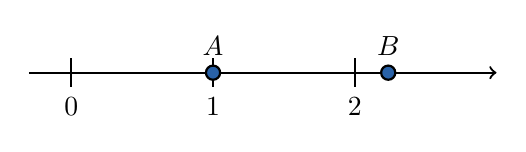
\begin{tikzpicture}[scale=1.8]
  \draw[thick, ->] (-0.3,0) -- (3,0);
  \draw[thick] (0, 0.1) -- (0, -0.1) node[below] {$0$};
  \draw[thick] (1, 0.1) -- (1, -0.1) node[below] {$1$};
  \draw[thick] (2, 0.1) -- (2, -0.1) node[below] {$2$};
  \draw[thick, fill=mainblue] (1, 0) circle (0.05);
  \node[above] at (1, 0.05) {$A$};
  \draw[thick, fill=mainblue] (2.236, 0) circle (0.05);
  \node[above] at (2.236, 0.05) {$B$};
\end{tikzpicture}
\end{center}
\end{examplebox}

\textbf{解}：

$A$ 点对应实数 $1$，$B$ 点对应实数 $\sqrt{5}$。

$C$ 是 $AB$ 的中点，所以 $C$ 点对应的实数为：
\[
C = \frac{1 + \sqrt{5}}{2}
\]

这恰好是\textbf{黄金比例} $\varphi \approx 1.618$。

% =============================================================
% 第三部分：应用题
% =============================================================
\section*{\textcolor{apppurple}{三、应用题}}

\begin{appbox}[【应用1】正方形面积与边长]
一个正方形的面积为 $20\text{ cm}^2$，求它的边长（用根号表示），并估算边长精确到 $0.1\text{ cm}$。
\end{appbox}

\textbf{解}：

设正方形的边长为 $a$，则 $a^2 = 20$。

所以 $a = \sqrt{20} = \sqrt{4 \times 5} = 2\sqrt{5}$（cm）。

估算：因为 $4^2 = 16 < 20 < 25 = 5^2$，所以 $4 < \sqrt{20} < 5$。

又 $4.4^2 = 19.36$，$4.5^2 = 20.25$，所以 $\sqrt{20} \approx 4.5$。

答：正方形的边长为 $2\sqrt{5}\text{ cm}$，约 $4.5\text{ cm}$。

\vspace{6pt}

\begin{appbox}[【应用2】立方体体积问题]
一个立方体的体积为 $64\text{ cm}^3$，求它的棱长。如果体积变为 $125\text{ cm}^3$ 呢？
\end{appbox}

\textbf{解}：

\begin{itemize}[leftmargin=2em]
  \item 体积 $V = 64\text{ cm}^3$ 时，棱长 $a = \sqrt[3]{64} = 4\text{ cm}$。
  \item 体积 $V = 125\text{ cm}^3$ 时，棱长 $a = \sqrt[3]{125} = 5\text{ cm}$。
\end{itemize}

答：体积为 $64\text{ cm}^3$ 时棱长为 $4\text{ cm}$；体积为 $125\text{ cm}^3$ 时棱长为 $5\text{ cm}$。

\vspace{6pt}

\begin{appbox}[【应用3】自由落体中的平方根]
一个物体从高处自由下落，下落距离 $h$（米）与时间 $t$（秒）的关系为 $h = 5t^2$。若物体下落了 $80$ 米，求下落时间 $t$。
\end{appbox}

\textbf{解}：

由 $h = 5t^2$，代入 $h = 80$：

\[
80 = 5t^2
\]
\[
t^2 = 16
\]
\[
t = \sqrt{16} = 4 \quad (\text{时间取正值})
\]

答：物体下落了 $80$ 米需要 $4$ 秒。

\vspace{6pt}

\begin{appbox}[【应用4】比较大小的实际应用]
小明家到学校有两条路线：路线 A 是沿正东走 $3$ 千米再沿正北走 $2$ 千米；路线 B 是走直线（沿东北方向）。请问路线 B 的距离是多少？（用根号表示，再估算）
\end{appbox}

\textbf{解}：

路线 A 形成一个直角三角形，东西方向 $3$ 千米，南北方向 $2$ 千米。

路线 B 是斜边，由勾股定理：
\[
\text{路线 B} = \sqrt{3^2 + 2^2} = \sqrt{9 + 4} = \sqrt{13} \text{ (千米)}
\]

估算：$3^2 = 9 < 13 < 16 = 4^2$，所以 $3 < \sqrt{13} < 4$。

$3.6^2 = 12.96$，$3.7^2 = 13.69$，所以 $\sqrt{13} \approx 3.6$ 千米。

答：路线 B 的距离为 $\sqrt{13}$ 千米，约 $3.6$ 千米。

% =============================================================
% 第四部分：课堂练习
% =============================================================
\section*{\textcolor{tipgreen}{四、课堂练习}}

\begin{enumerate}[leftmargin=2em]
  \item 求下列各数的平方根和算术平方根：
  \begin{enumerate}[label=(\arabic*)]
    \item $81$
    \item $0.36$
    \item $\dfrac{9}{16}$
  \end{enumerate}

  \item 求下列各数的立方根：
  \begin{enumerate}[label=(\arabic*)]
    \item $125$
    \item $-27$
    \item $-0.008$
  \end{enumerate}

  \item 判断下列各数哪些是有理数，哪些是无理数：
  \[
  -5,\quad \sqrt{11},\quad \frac{1}{3},\quad \pi - 3,\quad \sqrt[3]{8},\quad 0.123456\ldots\text{（不循环）}
  \]

  \item 估算 $\sqrt{50}$ 的值（精确到个位），并在数轴上大致标出其位置。

  \item 计算：
  \begin{enumerate}[label=(\arabic*)]
    \item $\sqrt{27} - 3\sqrt{\dfrac{1}{3}} + \sqrt{12}$
    \item $|2 - \sqrt{5}| + \sqrt{5}$
  \end{enumerate}
\end{enumerate}

\vspace{10pt}
\begin{knowledgebox}[参考答案]
\begin{enumerate}[leftmargin=2em]
  \item \begin{enumerate}[label=(\arabic*)]
    \item $81$ 的平方根为 $\pm 9$，算术平方根为 $9$。
    \item $0.36$ 的平方根为 $\pm 0.6$，算术平方根为 $0.6$。
    \item $\dfrac{9}{16}$ 的平方根为 $\pm\dfrac{3}{4}$，算术平方根为 $\dfrac{3}{4}$。
  \end{enumerate}

  \item \begin{enumerate}[label=(\arabic*)]
    \item $\sqrt[3]{125} = 5$
    \item $\sqrt[3]{-27} = -3$
    \item $\sqrt[3]{-0.008} = -0.2$
  \end{enumerate}

  \item \textbf{有理数}：$-5$，$\dfrac{1}{3}$，$\sqrt[3]{8} = 2$。

  \textbf{无理数}：$\sqrt{11}$，$\pi - 3$，$0.123456\ldots$（不循环）。

  \item $7^2 = 49 < 50 < 64 = 8^2$，所以 $7 < \sqrt{50} < 8$。$7.1^2 = 50.41 > 50$，所以 $\sqrt{50} \approx 7$（精确到个位）。

  \item \begin{enumerate}[label=(\arabic*)]
    \item $\sqrt{27} - 3\sqrt{\dfrac{1}{3}} + \sqrt{12} = 3\sqrt{3} - 3 \cdot \dfrac{\sqrt{3}}{3} + 2\sqrt{3} = 3\sqrt{3} - \sqrt{3} + 2\sqrt{3} = 4\sqrt{3}$

    \item $|2 - \sqrt{5}| + \sqrt{5} = (\sqrt{5} - 2) + \sqrt{5} = 2\sqrt{5} - 2$（因为 $\sqrt{5} > 2$，所以 $2 - \sqrt{5} < 0$）
  \end{enumerate}
\end{enumerate}
\end{knowledgebox}

\vfill
\begin{center}
\small\textcolor{gray}{本讲义仅供教学参考，例题可根据学生水平调整难度。}
\end{center}

\end{document}
